(Review of Long Division):\footnote{For more review, see Section \ref{polylongdiv}.}  In Exercises \ref{longpolydivreviewfirst} - \ref{longpolydivreviewlast}, use polynomial long division to perform the indicated division.  Write the polynomial in the form $p(x) = d(x)q(x) + r(x)$.

\begin{multicols}{2}
\begin{enumerate}
\item $\left(4x^2+3x-1 \right) \div (x-3)$ \label{longpolydivreviewfirst}
\item $\left(2x^3-x+1 \right) \div \left(x^{2} +x+1 \right)$

\setcounter{HW}{\value{enumi}}
\end{enumerate}
\end{multicols}

\begin{multicols}{2}
\begin{enumerate}
\setcounter{enumi}{\value{HW}}

\item $\left(5x^{4} - 3x^{3} + 2x^{2} - 1 \right) \div \left(x^{2} + 4 \right)$
\item $\left(-x^{5} + 7x^{3} - x \right) \div \left(x^{3} - x^{2} + 1 \right)$

\setcounter{HW}{\value{enumi}}
\end{enumerate}
\end{multicols}

\begin{multicols}{2}
\begin{enumerate}
\setcounter{enumi}{\value{HW}}

\item $\left(9x^{3} + 5 \right) \div \left(2x - 3 \right)$
\item $\left(4x^2 - x - 23 \right) \div \left(x^{2} - 1 \right)$ \label{longpolydivreviewlast}

\setcounter{HW}{\value{enumi}}
\end{enumerate}
\end{multicols}


In Exercises \ref{rationaltransfirst} - \ref{rationaltranslast}, given the pair of functions $f$ and $F$, sketch the graph of $y=F(x)$ by starting with the graph of $y = f(x)$ and using Theorem \ref{linearlaurentlgraphs}.   Track at least two points and the asymptotes.  State the domain and range using interval notation.


\begin{multicols}{2}
\begin{enumerate}
\setcounter{enumi}{\value{HW}}
\item $f(x) = \dfrac{1}{x}$,  $F(x) = \dfrac{1}{x-2}+1$ \label{rationaltransfirst}
\item $f(x) =\dfrac{1}{x}$, $F(x) = \dfrac{2x}{x+1}$

\setcounter{HW}{\value{enumi}}
\end{enumerate}
\end{multicols}

\begin{multicols}{2}
\begin{enumerate}
\setcounter{enumi}{\value{HW}}

\item $f(x) =x^{-1}$, $F(x)=4x(2x+1)^{-1}$
\item $f(x) = x^{-2}$, $F(x)=-(x-1)^{-2}+3$  \label{rationaltranslast}

\setcounter{HW}{\value{enumi}}
\end{enumerate}
\end{multicols}


In Exercises \ref{findformulafor1overxgraphfirst} - \ref{findformulafor1overxgraphlast}, find a formula for each function below in the form $F(x) = \dfrac{a}{x-h}+k$.

\begin{multicols}{2}

\begin{enumerate}
\setcounter{enumi}{\value{HW}}

\item $~$ \label{findformulafor1overxgraphfirst}  $y=F(x)$ %$F(x) = \dfrac{1}{x+2}-1$

\begin{mfpic}[15]{-5}{5}{-5}{5}
\axes
\tlabel[cc](5,-0.5){\scriptsize $x$}
\tlabel[cc](0.5,5){\scriptsize $y$}
%\tlabel[cc](-1.5, 0.5){\scriptsize $(-1,0)$}
%\tlabel[cc](-0.5,-1){\scriptsize $\left(0, \frac{1}{2} \right)$}
\xmarks{-4,-3,-2,-1,1,2,3,4}
\ymarks{-4,-3,-2, -1, 1,2,3,4}
\tlpointsep{4pt}
\scriptsize
\axislabels {x}{ {$-4 \hspace{7pt}$} -4, {$-3 \hspace{7pt}$} -3, {$-2 \hspace{7pt}$} -2, {$-1 \hspace{7pt}$} -1, {$1$} 1, {$2$} 2, {$3$} 3, {$4$} 4}
\axislabels {y}{{$-1$} -1,{$1$} 1, {$2$} 2, {$3$} 3, {$4$} 4, {$-2$} -2, {$-3$} -3, {$-4$} -4}
\dashed \polyline{(-4.75,-1), (4.75,-1)}
\dashed \polyline{(-2,-4.75), (-2,4.75)}
\penwd{1.25pt}
\arrow \reverse \arrow \function{-5,-2.25,0.1}{1/(x+2)-1}
\arrow \reverse \arrow \function{-1.83,5,0.1}{1/(x+2)-1}
\point[4pt]{(-1,0), (0,-0.5)}
\tcaption{ \scriptsize $x$-intercept $(-1,0)$, $y$-intercept $\left(0, -\frac{1}{2}\right)$}
\normalsize
\end{mfpic}



\item $~$ \label{findformulafor1overxgraphlast} $y = F(x)$ %$F(x) = -\dfrac{2}{x-1}+1$

\begin{mfpic}[15]{-5}{5}{-5}{5}
\axes
\tlabel[cc](5,-0.5){\scriptsize $x$}
\tlabel[cc](0.5,5){\scriptsize $y$}
%\tlabel[cc](-1.5, 0.5){\scriptsize $(-1,0)$}
%\tlabel[cc](-0.5,-1){\scriptsize $\left(0, \frac{1}{2} \right)$}
\xmarks{-4,-3,-2,-1,1,2,3,4}
\ymarks{-4,-3,-2, -1, 1,2,3,4}
\tlpointsep{4pt}
\scriptsize
\axislabels {x}{ {$-4 \hspace{7pt}$} -4, {$-3 \hspace{7pt}$} -3, {$-2 \hspace{7pt}$} -2, {$-1 \hspace{7pt}$} -1, {$1$} 1, {$2$} 2, {$3$} 3, {$4$} 4}
\axislabels {y}{{$-1$} -1,{$1$} 1, {$2$} 2, {$3$} 3, {$4$} 4, {$-2$} -2, {$-3$} -3, {$-4$} -4}
\dashed \polyline{(-4.75,1), (4.75,1)}
\dashed \polyline{(1,-4.75), (1,4.75)}
\penwd{1.25pt}
\arrow \reverse \arrow \function{-5,0.45,0.1}{1-2/(x-1)}
\arrow \reverse \arrow \function{1.35,5,0.1}{1-2/(x-1)}
\point[4pt]{(3,0), (0,3)}
\tcaption{ \scriptsize $x$-intercept $(3,0)$, $y$-intercept $\left(0, 3 \right)$}
\normalsize
\end{mfpic}


\setcounter{HW}{\value{enumi}}

\end{enumerate}

\end{multicols}

\newpage

In Exercises \ref{findformulafor1overxsquaredgraphfirst} - \ref{findformula1overxsquaredgraphlast}, find a formula for each function below in the form $F(x) = \dfrac{a}{(x-h)^2}+k$.


\begin{multicols}{2}

\begin{enumerate}

\setcounter{enumi}{\value{HW}}

\item $~$ \label{findformulafor1overxsquaredgraphfirst} $y = F(x)$ %$F(x) = -\dfrac{4}{(x+2)^2}+4$

\begin{mfpic}[15]{-5}{5}{-5}{5}
\axes
\tlabel[cc](5,-0.5){\scriptsize $x$}
\tlabel[cc](0.5,5){\scriptsize $y$}
%\tlabel[cc](-1.5, 0.5){\scriptsize $(-1,0)$}
%\tlabel[cc](-0.5,-1){\scriptsize $\left(0, \frac{1}{2} \right)$}
\xmarks{-4,-3,-2,-1,1,2,3,4}
\ymarks{-4,-3,-2, -1, 1,2,3,4}
\tlpointsep{4pt}
\scriptsize
\axislabels {x}{ {$-4 \hspace{7pt}$} -4,{$-2 \hspace{7pt}$} -2,  {$1$} 1, {$2$} 2, {$3$} 3, {$4$} 4}
\axislabels {y}{{$-1$} -1,{$1$} 1, {$2$} 2, {$3$} 3, {$4$} 4, {$-2$} -2, {$-3$} -3, {$-4$} -4}
\dashed \polyline{(-4.75,4), (4.75,4)}
\dashed \polyline{(-2,-4.75), (-2,4.75)}
\penwd{1.25pt}
\arrow \reverse \arrow \function{-5,-2.7,0.1}{4-4/((x+2)**2)}
\arrow \reverse \arrow \function{-1.3,5,0.1}{4-4/((x+2)**2)}
\point[4pt]{(-3,0), (-1,0), (0,3)}
\tcaption{\scriptsize $x$-intercepts $(-3,0)$,  $(-1,0)$, $y$-intercept $(0,3)$}
\normalsize
\end{mfpic}


\item $~$  \label{findformula1overxsquaredgraphlast}$y = F(x)$ %$F(x) = \dfrac{4}{(2x-1)^2}-4$

\begin{mfpic}[15]{-5}{5}{-5}{5}
\axes
\tlabel[cc](5,-0.5){\scriptsize $x$}
\tlabel[cc](0.5,5){\scriptsize $y$}
%\tlabel[cc](-1.5, 0.5){\scriptsize $(-1,0)$}
%\tlabel[cc](-0.5,-1){\scriptsize $\left(0, \frac{1}{2} \right)$}
\xmarks{-4,-3,-2,-1,1,2,3,4}
\ymarks{-4,-3,-2, -1, 1,2,3,4}
\tlpointsep{4pt}
\scriptsize
\axislabels {x}{ {$-4 \hspace{7pt}$} -4, {$-3 \hspace{7pt}$} -3, {$-2 \hspace{7pt}$} -2, {$-1 \hspace{7pt}$} -1, {$1$} 1, {$2$} 2, {$3$} 3, {$4$} 4}
\axislabels {y}{{$-1$} -1,{$1$} 1, {$2$} 2, {$3$} 3, {$4$} 4, {$-2$} -2, {$-4$} -4}
\dashed \polyline{(-4.75,-4), (4.75,-4)}
\dashed \polyline{(0.5,-4.75), (0.5,4.75)}
\penwd{1.25pt}
\arrow \reverse \arrow \function{-5, 0.16, 0.1}{4/((2*x-1)**2) - 4}
\arrow \reverse \arrow \function{0.84, 5, 0.1}{4/((2*x-1)**2) - 4}
\point[4pt]{(0,0), (1,0)}
\tcaption{\scriptsize $x$-intercepts $(0,0)$,  $(1,0)$, Vertical Asymptote:  $x = \frac{1}{2}$}
\normalsize
\end{mfpic}



\setcounter{HW}{\value{enumi}}

\end{enumerate}

\end{multicols}



In Exercises \ref{alltheasympfirst} - \ref{alltheasymplast}, for the given rational function:

\begin{multicols}{2}
\begin{itemize}

\item State the domain.
\item Identify any vertical asymptotes of the graph.

\end{itemize}
\end{multicols}

\begin{multicols}{2}
\begin{itemize}

\item Identify any holes in the graph.
\item Find the horizontal asymptote, if it exists.

\end{itemize}
\end{multicols}

\begin{multicols}{2}
\begin{itemize}

\item Find the slant asymptote, if it exists.
\item Graph the function using a graphing utility and describe the behavior near the asymptotes.

\end{itemize}
\end{multicols}

\begin{multicols}{3}
\begin{enumerate}
\setcounter{enumi}{\value{HW}}

\item $f(x) = \dfrac{x}{3x - 6}$ \label{alltheasympfirst}
\item $f(x) = \dfrac{3 + 7x}{5 - 2x}$
\item $f(x) = \dfrac{x}{x^{2} + x - 12}$

\setcounter{HW}{\value{enumi}}
\end{enumerate}
\end{multicols}

\begin{multicols}{3}
\begin{enumerate}
\setcounter{enumi}{\value{HW}}

\item $g(t) = \dfrac{t}{t^{2} + 1}$
\item $g(t) = \dfrac{t + 7}{(t + 3)^{2}}$
\item $g(t) = \dfrac{t^{3} + 1}{t^{2} - 1}$

\setcounter{HW}{\value{enumi}}
\end{enumerate}
\end{multicols}

\begin{multicols}{3}
\begin{enumerate}
\setcounter{enumi}{\value{HW}}

\item $r(z) = \dfrac{4z}{z^2+4}$
\item $r(z) = \dfrac{4z}{z^2-4}$
\item $r(z) = \dfrac{z^2-z-12}{z^2+z-6}$

\setcounter{HW}{\value{enumi}}
\end{enumerate}
\end{multicols}

\begin{multicols}{3}
\begin{enumerate}
\setcounter{enumi}{\value{HW}}

\item $f(x) = \dfrac{3x^2-5x-2}{x^2-9}$
\item $f(x) = \dfrac{x^3+2x^2+x}{x^2-x-2}$
\item $f(x) = \dfrac{x^{3} - 3x + 1}{x^{2} + 1}$

\setcounter{HW}{\value{enumi}}
\end{enumerate}
\end{multicols}

\begin{multicols}{3}
\begin{enumerate}
\setcounter{enumi}{\value{HW}}

\item $g(t) = \dfrac{2t^{2} + 5t - 3}{3t + 2}$
\item $g(t) = \dfrac{-t^{3} + 4t}{t^{2} - 9}$
\item \small $g(t) = \dfrac{-5t^{4} - 3t^{3} + t^{2} - 10}{t^{3} - 3t^{2} + 3t - 1}$ \normalsize

\setcounter{HW}{\value{enumi}}
\end{enumerate}
\end{multicols}


\begin{multicols}{3}
\begin{enumerate}
\setcounter{enumi}{\value{HW}}

\item $r(z) = \dfrac{z^3}{1-z}$
\item $r(z) = \dfrac{18-2z^2}{z^2-9}$
\item $r(z) = \dfrac{z^3-4z^2-4z-5}{z^2+z+1}$ \label{alltheasymplast}


\setcounter{HW}{\value{enumi}}
\end{enumerate}
\end{multicols}

\newpage

\begin{enumerate}
\setcounter{enumi}{\value{HW}}



\item The cost $C(p)$ in dollars to remove $p$\% of the invasive  Ippizuti fish species from Sasquatch Pond is: \[C(p) = \frac{1770p}{100 - p}, \quad 0 \leq p < 100 \]

\begin{enumerate}

\item Find and interpret $C(25)$ and $C(95)$.
\item What does the vertical asymptote at $x = 100$ mean within the context of the problem?
\item What percentage of the Ippizuti fish can you remove for  \$40000?

\end{enumerate}

\item  In the scenario of  Example \ref{averagevelocityrocketex}, $s(t) = -5t^2+100t$, $0 \leq t \leq 20$ gives the height of a model rocket above the Moon's surface, in feet,  $t$ seconds after liftoff.  For each of the times $t_{0}$ listed below, find and simplify a the formula for the average velocity $\overline{v}(t)$ between $t$ and $t_{0}$ (see Definition \ref{averagevelocitydefn}) and use $\overline{v}(t)$ to find and interpret the instantaneous velocity of the rocket at $t = t_{0}$.

\begin{multicols}{4}

\begin{enumerate}

\item  $t_{0} = 5$

\item $t_{0} = 9$

\item $t_{0} = 10$

\item  $t_{0} = 11$

\end{enumerate}

\end{multicols}


\item \label{squatchpop} The population of Sasquatch in Portage County $t$ years after the year 1803 is modeled by the function \[P(t) = \frac{150t}{t + 15}.\] Find and interpret the horizontal asymptote of the graph of $y = P(t)$ and explain what it means.

\item  The cost in dollars, $C(x)$ to make $x$ dOpi media players is $C(x) = 100x+2000$, $x \geq 0$.  You may wish to review the concepts of fixed and variable costs introduced in  Example \ref{PortaBoyCost} in Section \ref{LinearFunctions}.

\begin{enumerate}

\item  Find a formula for the average cost $\overline{C}(x)$.

\item  Find and interpret $\overline{C}(1)$ and $\overline{C}(100)$.

\item  How many dOpis need to be produced so that the average cost per dOpi is $\$ 200$?

\item  Interpret the behavior of $\overline{C}(x)$ as $x \rightarrow 0^{+}$.

\item  Interpret the behavior of $\overline{C}(x)$ as $x \rightarrow \infty$.

\end{enumerate}

\item  \label{averagevariablecostexercise}   This exercise explores the relationships between fixed cost, variable cost, and average cost.  The reader is encouraged to revisit Example \ref{PortaBoyCost} in Section \ref{LinearFunctions} as needed.  Suppose the cost in dollars $C(x)$ to make $x$ items is given by $C(x) = mx + b$ where $m$ and $b$ are positive real numbers.

\begin{enumerate}

\item  Show the fixed cost (the money spent even if no items are made) is $b$.
\item  Show the variable cost (the increase in cost per item made) is $m$.
\item  Find a formula for the average cost when making $x$ items, $\overline{C}(x)$.
\item  Show $\overline{C}(x) > m$ for all $x>0$ and, moreover,   $\overline{C}(x)  \rightarrow m^{+}$ as $x \rightarrow \infty$.
\item  Interpret $\overline{C}(x)  \rightarrow m^{+}$ both geometrically and in terms of fixed, variable, and average costs.

\end{enumerate}

\item  \label{slantyintaverageprofitexercise} Suppose the price-demand function for a particular product is given by $p(x) = mx + b$  where $x$ is the number of items made and sold for $p(x)$ dollars.  Here,  $m<0$ and $b>0$.  If the cost (in dollars) to make $x$ of these products is also a linear  function $C(x)$, show that the graph of the average profit function $\overline{P}(x)$ has a slant asymptote with slope $m$ and interpret.

\item In Exercise \ref{circuitexercisepoly} in Section \ref{GraphsofPolynomials}, we fit a few polynomial models to the following electric circuit data. The circuit was built with a variable resistor.  For each of the following resistance values (measured in kilo-ohms, $k \Omega$),  the corresponding power to the load (measured in milliwatts, $mW$) is given below.\footnote{The authors wish to thank Don Anthan and Ken White of Lakeland Community College for devising this problem and generating the accompanying data set.}


\smallskip

\noindent \begin{tabular}{|l|r|r|r|r|r|r|} \hline
Resistance: ($k \Omega$) & 1.012 & 2.199 & 3.275 & 4.676 & 6.805 & 9.975 \\ \hline
Power: ($mW$) & 1.063 & 1.496 & 1.610 & 1.613 & 1.505 & 1.314 \\ \hline
\end{tabular}

\smallskip

\noindent Using some fundamental laws of circuit analysis mixed with a healthy dose of algebra, we can derive the actual formula relating power $P(x)$ to resistance $x$:   \[P(x) = \frac{25x}{(x + 3.9)^2}, \quad x \geq 0.\]

\begin{enumerate}

\item Graph the data along with the function $y = P(x)$ using a graphing utility.

\item Use a graphing utility to approximate the maximum power that can be delivered to the load.  What is the corresponding resistance value?

\item Find and interpret the end behavior of $P(x)$ as $x \rightarrow \infty$.

\end{enumerate}


\item  Let $f(x) = \dfrac{ax^2-c}{x+3}$.  Find values  for $a$ and  $c$ so  the graph of $f$ has a hole  at $(-3, 12)$.

\item  Let  $f(x) = \dfrac{ax^{n} -4}{2x^2+1}$.

\begin{enumerate}

\item  Find values for $a$ and $n$ so the graph of $y = f(x)$  has the horizontal asymptote $y = 3$.

\item  Find values for $a$ and $n$ so the graph of  $y=f(x)$ has the slant asymptote $y = 5x$.

\end{enumerate}


\item  Suppose $p$ is a polynomial function and $a$ is a real number.  Define $r(x)= \dfrac{p(x) - p(a)}{x-a}$.  Use the Factor Theorem, Theorem \ref{factorthm}, to prove the graph of $y = r(x)$ has a hole at $x =a$.


\item \label{laurentarcexercise}For each function $f(x)$ listed below, compute the average rate of change over the indicated interval.\footnote{See Definition \ref{arc} in Section \ref{AverageRateofChange} for a review of this concept, as needed.}  What trends do you observe?  How do your answers manifest themselves graphically?  How do you results compare with those of Exercise \ref{monomialarcexercise} in Section \ref{GraphsofPolynomials}?

\vspace*{-0.2in}

\[ \begin{array}{|r||c|c|c|c|}  \hline

 f(x) &  [0.9, 1.1] & [0.99, 1.01] &[0.999, 1.001] & [0.9999, 1.0001]  \\ \hline
 x^{-1} &&&&   \\  \hline
 x^{-2} &&&&    \\  \hline
 x^{-3} &&&&   \\  \hline
 x^{-4} &&&&   \\  \hline
\end{array} \]

\item \index{Learning Curve Equation} \index{Thurstone, Louis Leon} In his now famous 1919 dissertation \underline{The Learning Curve Equation}, Louis Leon Thurstone presents a rational function which models the number of words a person can type in four minutes as a function of the number of pages of practice one has completed.\footnote{This paper, which is now in the public domain and can be found  \href{http://bit.ly/2uNaUBa}{\underline{here}}, is from a bygone era when students at business schools took typing classes on manual typewriters.} Using his original notation and original language, we have $Y = \frac{L(X + P)}{(X + P) + R}$ where $L$ is the predicted practice limit in terms of speed units, $X$ is pages written, $Y$ is writing speed in terms of words in four minutes, $P$ is equivalent previous practice in terms of pages and $R$ is the rate of learning. In Figure 5 of the paper, he graphs a scatter plot and the curve $Y = \frac{216(X + 19)}{X + 148}$.  Discuss this equation with your classmates.  How would you update the notation?  Explain what the horizontal asymptote of the graph means.  You should take some time to look at the original paper. Skip over the computations you don't understand yet and try to get a sense of the time and place in which the study was conducted.

\end{enumerate}

\newpage

\subsection{Answers}

\begin{enumerate}
\item $4x^2+3x-1 = (x-3)(4x+15) + 44$
\item $2x^3-x+1 = \left(x^2+x+1\right)(2x-2)+(-x+3)$
\item $5x^{4} - 3x^{3} + 2x^{2} - 1 = \left(x^{2} + 4 \right) \left(5x^{2} - 3x - 18 \right) + (12x + 71)$
\item $-x^{5} + 7x^{3} - x = \left(x^{3} - x^{2} + 1 \right) \left(-x^{2} - x + 6 \right) + \left(7x^{2} - 6 \right)$
\item $9x^{3} + 5 =(2x - 3) \left(\frac{9}{2}x^{2} + \frac{27}{4}x + \frac{81}{8} \right) + \frac{283}{8}$
\item $4x^2 - x - 23 = \left(x^{2} - 1 \right)(4) + (-x - 19)$
\setcounter{HW}{\value{enumi}}
\end{enumerate}


\begin{multicols}{2}
\begin{enumerate}
\setcounter{enumi}{\value{HW}}

\item $F(x) = \dfrac{1}{x-2}+1$ \\ [10pt]
Domain: $(-\infty, 2) \cup (2, \infty)$ \\
Range: $(-\infty, 1) \cup (1, \infty)$ \\
Vertical asymptote:  $x = 2$\\
Horizontal asymptote:  $y = 1$ \\

\begin{mfpic}[15]{-5}{5}{-5}{5}
\axes
\tlabel[cc](5,-0.5){\scriptsize $x$}
\tlabel[cc](0.5,5){\scriptsize $y$}
%\tlabel[cc](-1.5, 0.5){\scriptsize $(-1,0)$}
%\tlabel[cc](-0.5,-1){\scriptsize $\left(0, \frac{1}{2} \right)$}
\xmarks{-4,-3,-2,-1,1,2,3,4}
\ymarks{-4,-3,-2, -1, 1,2,3,4}
\tlpointsep{4pt}
\scriptsize
\axislabels {x}{ {$-4 \hspace{7pt}$} -4, {$-3 \hspace{7pt}$} -3, {$-2 \hspace{7pt}$} -2, {$-1 \hspace{7pt}$} -1, {$1$} 1, {$2$} 2, {$3$} 3, {$4$} 4}
\axislabels {y}{{$-1$} -1,{$1$} 1, {$2$} 2, {$3$} 3, {$4$} 4, {$-2$} -2, {$-3$} -3, {$-4$} -4}
\dashed \polyline{(-4.75,1), (4.75,1)}
\dashed \polyline{(2,-4.75), (2,4.75)}
\penwd{1.25pt}
\arrow \reverse \arrow \function{-5,1.8,0.1}{1+1/(x-2)}
\arrow \reverse \arrow \function{2.3,5,0.1}{1+1/(x-2)}
\point[4pt]{(1,0), (3,2)}
\normalsize
\end{mfpic}


\vfill

\columnbreak

\item $F(x) = \dfrac{2x}{x+1} = \dfrac{-2}{x+1}+2$\\ [10pt]
Domain: $(-\infty, -1) \cup (-1, \infty)$ \\
Range: $(-\infty, 2) \cup (2, \infty)$ \\
Vertical asymptote:  $x = -1$\\
Horizontal asymptote:  $y = 2$ \\

\begin{mfpic}[15]{-5}{5}{-5}{5}
\axes
\tlabel[cc](5,-0.5){\scriptsize $x$}
\tlabel[cc](0.5,5){\scriptsize $y$}
%\tlabel[cc](-1.5, 0.5){\scriptsize $(-1,0)$}
%\tlabel[cc](-0.5,-1){\scriptsize $\left(0, \frac{1}{2} \right)$}
\xmarks{-4,-3,-2,-1,1,2,3,4}
\ymarks{-4,-3,-2, -1, 1,2,3,4}
\tlpointsep{4pt}
\scriptsize
\axislabels {x}{ {$-4 \hspace{7pt}$} -4, {$-3 \hspace{7pt}$} -3, {$-2 \hspace{7pt}$} -2, {$-1 \hspace{7pt}$} -1, {$1$} 1, {$2$} 2, {$3$} 3, {$4$} 4}
\axislabels {y}{{$1$} 1, {$2$} 2, {$3$} 3, {$4$} 4}
\dashed \polyline{(-4.75,2), (4.75,2)}
\dashed \polyline{(-1,-4.75), (-1,4.75)}
\penwd{1.25pt}
\arrow \reverse \arrow \function{-5,-1.7,0.1}{2x/(x+1)}
\arrow \reverse \arrow \function{-0.7,5,0.1}{2x/(x+1)}
\point[4pt]{(0,0), (-2,4)}
\normalsize
\end{mfpic}

\setcounter{HW}{\value{enumi}}
\end{enumerate}
\end{multicols}



\begin{multicols}{2}
\begin{enumerate}
\setcounter{enumi}{\value{HW}}

\item $F(x)=4x(2x+1)^{-1} = \dfrac{4x}{2x+1} = \dfrac{-1}{x+\frac{1}{2}}+2$ \\ [10pt]
Domain: $\left(-\infty, -\frac{1}{2} \right) \cup \left(-\frac{1}{2},  \infty \right)$ \\
Range: $(-\infty, 2) \cup (2, \infty)$ \\
Vertical asymptote:  $x  = -\frac{1}{2}$ \\
Horizontal asymptote: $y= 2$\\ 

\begin{mfpic}[15]{-5}{5}{-5}{5}
\axes
\tlabel[cc](5,-0.5){\scriptsize $x$}
\tlabel[cc](0.5,5){\scriptsize $y$}
%\tlabel[cc](-1.5, 0.5){\scriptsize $(-1,0)$}
%\tlabel[cc](-0.5,-1){\scriptsize $\left(0, \frac{1}{2} \right)$}
\xmarks{-4,-3,-2,-1,1,2,3,4}
\ymarks{-4,-3,-2, -1, 1,2,3,4}
\tlpointsep{4pt}
\scriptsize
\axislabels {x}{ {$-4 \hspace{7pt}$} -4, {$-3 \hspace{7pt}$} -3, {$-2 \hspace{7pt}$} -2, {$-1 \hspace{7pt}$} -1, {$1$} 1, {$2$} 2, {$3$} 3, {$4$} 4}
\axislabels {y}{{$1$} 1, {$2$} 2, {$3$} 3, {$4$} 4}
\dashed \polyline{(-4.75,2), (4.75,2)}
\dashed \polyline{(-0.5,-4.75), (-0.5,4.75)}
\penwd{1.25pt}
\arrow \reverse \arrow \function{-5,-0.84,0.1}{4*x/(2*x+1)}
\arrow \reverse \arrow \function{-0.35,5,0.1}{4*x/(2*x+1)}
\point[4pt]{(-1.5,3), (0.5,1)}
\normalsize
\end{mfpic}


\vfill

\columnbreak

\item $F(x)=-(x-1)^{-2}+3 = \dfrac{-1}{(x-1)^2} + 3$\\[10pt]
Domain: $(-\infty, 1) \cup (1, \infty)$ \\
Range: $(-\infty, 3) \cup (3, \infty)$ \\
Vertical asymptote:  $x = 1$\\
Horizontal asymptote:  $y = 3$ \\

\begin{mfpic}[15]{-5}{5}{-5}{5}
\axes
\tlabel[cc](5,-0.5){\scriptsize $x$}
\tlabel[cc](0.5,5){\scriptsize $y$}
%\tlabel[cc](-1.5, 0.5){\scriptsize $(-1,0)$}
%\tlabel[cc](-0.5,-1){\scriptsize $\left(0, \frac{1}{2} \right)$}
\xmarks{-4,-3,-2,-1,1,2,3,4}
\ymarks{-4,-3,-2, -1, 1,2,3,4}
\tlpointsep{4pt}
\scriptsize
\axislabels {x}{ {$-4 \hspace{7pt}$} -4, {$-3 \hspace{7pt}$} -3, {$-2 \hspace{7pt}$} -2, {$-1 \hspace{7pt}$} -1,  {$2$} 2, {$3$} 3, {$4$} 4}
\axislabels {y}{{$1$} 1, {$2$} 2, {$3$} 3, {$4$} 4, {$-1$} -1, {$-2$} -2, {$-3$} -3, {$-4$} -4}
\dashed \polyline{(-4.75,3), (4.75,3)}
\dashed \polyline{(1,-4.75), (1,4.75)}
\penwd{1.25pt}
\arrow \reverse \arrow \function{-5,0.64,0.1}{3-1/((x-1)**2)}
\arrow \reverse \arrow \function{1.36,5,0.1}{3-1/((x-1)**2)}
\point[4pt]{(0,2), (2,2)}
\normalsize
\end{mfpic}

\setcounter{HW}{\value{enumi}}
\end{enumerate}
\end{multicols}

\begin{multicols}{2}
\begin{enumerate}
\setcounter{enumi}{\value{HW}}

\item $F(x) = \dfrac{1}{x+2}-1$

\item  $F(x) = \dfrac{-2}{x-1}+1$

\setcounter{HW}{\value{enumi}}
\end{enumerate}
\end{multicols}


\begin{multicols}{2}

\begin{enumerate}

\setcounter{enumi}{\value{HW}}

\item  $F(x) = \dfrac{-4}{(x+2)^2}+4$  \vphantom{$F(x) = \dfrac{1}{\left(x-\frac{1}{2}\right)^2}-4$}

\item $F(x) = \dfrac{1}{\left(x-\frac{1}{2}\right)^2}-4$

\setcounter{HW}{\value{enumi}}
\end{enumerate}
\end{multicols}



\begin{multicols}{2}
\begin{enumerate}
\setcounter{enumi}{\value{HW}}

\item $f(x) = \dfrac{x}{3x - 6}$ \vphantom{$\dfrac{7x}{7x}$}\\
Domain: $(-\infty, 2) \cup (2, \infty)$\\
Vertical asymptote: $x = 2$\\
As $x \rightarrow 2^{-}, f(x) \rightarrow -\infty$\\
As $x \rightarrow 2^{+}, f(x) \rightarrow \infty$\\
No holes in the graph\\
Horizontal asymptote: $y = \frac{1}{3}$ \\
As $x \rightarrow -\infty, f(x) \rightarrow \frac{1}{3}^{-}$\\
As $x \rightarrow \infty, f(x) \rightarrow \frac{1}{3}^{+}$\\

\vfill

\columnbreak

\item $f(x) = \dfrac{3 + 7x}{5 - 2x}$\\
Domain: $(-\infty, \frac{5}{2}) \cup (\frac{5}{2}, \infty)$\\
Vertical asymptote: $x = \frac{5}{2}$\\
As $x \rightarrow \frac{5}{2}^{-}, f(x) \rightarrow \infty$\\
As $x \rightarrow \frac{5}{2}^{+}, f(x) \rightarrow -\infty$\\
No holes in the graph\\
Horizontal asymptote: $y = -\frac{7}{2}$ \\
As $x \rightarrow -\infty, f(x) \rightarrow -\frac{7}{2}^{+}$\\
As $x \rightarrow \infty, f(x) \rightarrow -\frac{7}{2}^{-}$\\

\setcounter{HW}{\value{enumi}}
\end{enumerate}
\end{multicols}

\begin{multicols}{2}
\begin{enumerate}
\setcounter{enumi}{\value{HW}}

\item $f(x) = \dfrac{x}{x^{2} + x - 12} = \dfrac{x}{(x + 4)(x - 3)}$\\
Domain: $(-\infty, -4) \cup (-4, 3) \cup (3, \infty)$\\
Vertical asymptotes: $x = -4, x = 3$\\
As $x \rightarrow -4^{-}, f(x) \rightarrow -\infty$\\
As $x \rightarrow -4^{+}, f(x) \rightarrow \infty$\\
As $x \rightarrow 3^{-}, f(x) \rightarrow -\infty$\\
As $x \rightarrow 3^{+}, f(x) \rightarrow \infty$\\
No holes in the graph\\
Horizontal asymptote: $y = 0$ \\
As $x \rightarrow -\infty, f(x) \rightarrow 0^{-}$\\
As $x \rightarrow \infty, f(x) \rightarrow 0^{+}$\\

\vfill

\columnbreak


\item $g(t) = \dfrac{t}{t^{2} + 1}$\\
Domain: $(-\infty, \infty)$\\
No vertical asymptotes\\
No holes in the graph\\
Horizontal asymptote: $y = 0$ \\
As $t \rightarrow -\infty, g(t) \rightarrow 0^{-}$\\
As $t \rightarrow \infty, g(t) \rightarrow 0^{+}$\\

\setcounter{HW}{\value{enumi}}
\end{enumerate}
\end{multicols}

\begin{multicols}{2}
\begin{enumerate}
\setcounter{enumi}{\value{HW}}

\item $g(t) = \dfrac{t + 7}{(t + 3)^{2}}$ \vphantom{$\dfrac{t^{3}}{t^{2}}$}\\
Domain: $(-\infty, -3) \cup (-3, \infty)$\\
Vertical asymptote: $t = -3$\\
As $t \rightarrow -3^{-}, g(t) \rightarrow \infty$\\
As $t \rightarrow -3^{+}, g(t) \rightarrow \infty$\\
No holes in the graph\\
Horizontal asymptote: $y = 0$ \\
\footnote{This is hard to see on the calculator, but trust me, the graph is below the $t$-axis to the left of $t = -7$.}As $t \rightarrow -\infty, g(t) \rightarrow 0^{-}$\\
As $t \rightarrow \infty, g(t) \rightarrow 0^{+}$\\

\vfill

\columnbreak

\item $g(t) = \dfrac{t^{3} + 1}{t^{2} - 1} = \dfrac{t^{2} - t+ 1}{t-1}$\\
Domain: $(-\infty, -1) \cup (-1, 1) \cup (1, \infty)$\\
Vertical asymptote: $t = 1$\\
As $t \rightarrow 1^{-}, g(t) \rightarrow -\infty$\\
As $t \rightarrow 1^{+}, g(t) \rightarrow \infty$\\
Hole at $(-1, -\frac{3}{2})$\\
Slant asymptote: $y=t$  \\
As $t \rightarrow -\infty$, the graph is below $y=t$\\
As $t \rightarrow \infty$, the graph is above $y=t$\\

\setcounter{HW}{\value{enumi}}
\end{enumerate}
\end{multicols}

\begin{multicols}{2}
\begin{enumerate}
\setcounter{enumi}{\value{HW}}

\item $r(z) = \dfrac{4z}{z^{2} + 4}$\\
Domain: $(-\infty,  \infty)$\\
No vertical asymptotes \\
No holes in the graph\\
Horizontal asymptote: $y = 0$ \\
As $z \rightarrow -\infty, r(z) \rightarrow 0^{-}$\\
As $z \rightarrow \infty, r(z) \rightarrow 0^{+}$\\


\vfill

\columnbreak

\item $r(z) = \dfrac{4z}{z^{2} -4} = \dfrac{4z}{(z + 2)(z - 2)}$\\
Domain: $(-\infty, -2) \cup (-2, 2) \cup (2, \infty)$\\
Vertical asymptotes: $z = -2, z = 2$\\
As $z \rightarrow -2^{-}, r(z) \rightarrow -\infty$\\
As $z \rightarrow -2^{+}, r(z) \rightarrow \infty$\\
As $z \rightarrow 2^{-}, r(z) \rightarrow -\infty$\\
As $z \rightarrow 2^{+}, r(z) \rightarrow \infty$\\
No holes in the graph\\
Horizontal asymptote: $y = 0$ \\
As $z \rightarrow -\infty, r(z) \rightarrow 0^{-}$\\
As $z \rightarrow \infty, r(z) \rightarrow 0^{+}$\\

\setcounter{HW}{\value{enumi}}
\end{enumerate}
\end{multicols}

\begin{multicols}{2}
\begin{enumerate}
\setcounter{enumi}{\value{HW}}

\item $r(z) = \dfrac{z^2-z-12}{z^{2} +z - 6} = \dfrac{z-4}{z - 2}$\\
Domain: $(-\infty, -3) \cup (-3, 2) \cup (2, \infty)$\\
Vertical asymptote: $z = 2$\\
As $z \rightarrow 2^{-}, r(z) \rightarrow \infty$\\
As $z \rightarrow 2^{+}, r(z) \rightarrow -\infty$\\
Hole at $\left(-3, \frac{7}{5} \right)$ \\
Horizontal asymptote: $y = 1$ \\
As $z \rightarrow -\infty, r(z) \rightarrow 1^{+}$\\
As $z \rightarrow \infty, r(z) \rightarrow 1^{-}$\\


\vfill

\columnbreak

\item $f(x) = \dfrac{3x^2-5x-2}{x^{2} -9} = \dfrac{(3x+1)(x-2)}{(x + 3)(x - 3)}$\\
Domain: $(-\infty, -3) \cup (-3, 3) \cup (3, \infty)$\\
Vertical asymptotes: $x = -3, x = 3$\\
As $x \rightarrow -3^{-}, f(x) \rightarrow \infty$\\
As $x \rightarrow -3^{+}, f(x) \rightarrow -\infty$\\
As $x \rightarrow 3^{-}, f(x) \rightarrow -\infty$\\
As $x \rightarrow 3^{+}, f(x) \rightarrow \infty$\\
No holes in the graph\\
Horizontal asymptote: $y = 3$ \\
As $x \rightarrow -\infty, f(x) \rightarrow 3^{+}$\\
As $x \rightarrow \infty, f(x) \rightarrow 3^{-}$\\

\setcounter{HW}{\value{enumi}}
\end{enumerate}
\end{multicols}

\begin{multicols}{2}
\begin{enumerate}
\setcounter{enumi}{\value{HW}}


\item $f(x) = \dfrac{x^3+2x^2+x}{x^{2} -x-2} = \dfrac{x(x+1)}{x - 2}$\\
Domain: $(-\infty, -1) \cup (-1, 2) \cup (2, \infty)$\\
Vertical asymptote: $x = 2$\\
As $x \rightarrow 2^{-}, f(x) \rightarrow -\infty$\\
As $x \rightarrow 2^{+}, f(x) \rightarrow \infty$\\
Hole at $(-1,0)$ \\
Slant asymptote: $y=x+3$ \\
As $x \rightarrow -\infty$, the graph is below $y=x+3$\\
As $x \rightarrow \infty$, the graph is above $y=x+3$\\

\vfill

\columnbreak

\item $f(x) = \dfrac{x^3-3x+1}{x^2+1}$\\
Domain: $(-\infty, \infty)$\\
No vertical asymptotes \\
No holes in the graph \\
Slant asymptote: $y=x$ \\
As $x \rightarrow -\infty$, the graph is above $y=x$ \\
As $x \rightarrow \infty$, the graph is below $y=x$  \\


\setcounter{HW}{\value{enumi}}
\end{enumerate}
\end{multicols}


\begin{multicols}{2}
\begin{enumerate}
\setcounter{enumi}{\value{HW}}

\item $g(t) = \dfrac{2t^{2} + 5t - 3}{3t + 2}$\\
Domain: $\left(-\infty, -\frac{2}{3}\right) \cup \left(-\frac{2}{3}, \infty\right)$\\
Vertical asymptote: $t = -\frac{2}{3}$\\
As $t \rightarrow -\frac{2}{3}^{-}, g(t) \rightarrow \infty$\\
As $t \rightarrow -\frac{2}{3}^{+}, g(t) \rightarrow -\infty$\\
No holes in the graph \\
Slant asymptote:  $y = \frac{2}{3}t + \frac{11}{9}$ \\
As $t \rightarrow  -\infty$, the graph is above \small $y = \frac{2}{3}t + \frac{11}{9}$\\
\normalsize As $t \rightarrow \infty$, the graph is below \small $y = \frac{2}{3}t + \frac{11}{9}$ \normalsize \\

\vfill

\columnbreak

\item $g(t) = \dfrac{-t^{3} + 4t}{t^{2} - 9} = \dfrac{-t^{3} + 4t}{(t-3)(t+3)} $\\
Domain: $(-\infty, -3) \cup (-3, 3) \cup (3, \infty)$\\
Vertical asymptotes: $t = -3$, $t=3$\\
As $t \rightarrow -3^{-}, g(t) \rightarrow \infty$\\
As $t \rightarrow -3^{+}, g(t) \rightarrow -\infty$\\
As $t \rightarrow 3^{-}, g(t) \rightarrow \infty$\\
As $t \rightarrow 3^{+}, g(t) \rightarrow -\infty$\\
No holes in the graph \\
Slant asymptote: $y=-t$ \\
As $t \rightarrow -\infty$, the graph is above $y=-t$\\
As $t \rightarrow \infty$, the graph is below $y=-t$\\


\setcounter{HW}{\value{enumi}}
\end{enumerate}
\end{multicols}

\begin{multicols}{2}
\begin{enumerate}
\setcounter{enumi}{\value{HW}}

\item \small $g(t) = \dfrac{-5t^{4} - 3t^{3} + t^{2} - 10}{t^{3} - 3t^{2} + 3t - 1} \\ \phantom{g(t)} = \dfrac{-5t^{4} - 3t^{3} + t^{2} - 10}{(t-1)^3} $ \normalsize \\
Domain: $(-\infty, 1) \cup (1, \infty)$\\
Vertical asymptotes: $t = 1$\\
As $t \rightarrow 1^{-}, g(t) \rightarrow \infty$\\
As $t \rightarrow 1^{+}, g(t) \rightarrow -\infty$\\
No holes in the graph \\
Slant asymptote: $y=-5t-18$ \\
 \small  As $t \rightarrow -\infty$, the graph is above $y=-5t-18$ \normalsize\\
 \small  As $t \rightarrow \infty$, the graph is below $y=-5t-18$ \normalsize \\

 \vfill

 \columnbreak

\item $r(z) = \dfrac{z^3}{1-z}$\\
Domain: $(-\infty, 1) \cup (1, \infty)$\\
Vertical asymptote: $z=1$\\
As $z \rightarrow 1^{-}, r(z) \rightarrow \infty$\\
As $z \rightarrow 1^{+}, r(z) \rightarrow -\infty$\\
No holes in the graph \\
No horizontal or slant asymptote \\
As $z \rightarrow -\infty$, $r(z) \rightarrow -\infty$\\
As $z \rightarrow \infty$, $r(z) \rightarrow -\infty$\\


\setcounter{HW}{\value{enumi}}
\end{enumerate}
\end{multicols}

\begin{multicols}{2}
\begin{enumerate}
\setcounter{enumi}{\value{HW}}

\item $r(z) = \dfrac{18-2z^2}{z^2-9} = -2$\\
Domain: $(-\infty, -3) \cup (-3,3) \cup (3, \infty)$\\
No vertical asymptotes \\
Holes in the graph at $(-3,-2)$ and $(3,-2)$ \\
Horizontal asymptote $y = -2$ \\
As $z \rightarrow \pm \infty$, $r(z) = -2$ \\

\vfill
\columnbreak

\item $r(z) = \dfrac{z^3-4z^2-4z-5}{z^2+z+1} = z-5$\\
Domain: $(-\infty, \infty)$\\
No vertical asymptotes \\
No holes in the graph \\
Slant asymptote:  $y = z-5$ \\
$r(z) = z-5$ everywhere. \\


\setcounter{HW}{\value{enumi}}
\end{enumerate}
\end{multicols}

\begin{enumerate}
\setcounter{enumi}{\value{HW}}


\item \begin{enumerate}

\item $C(25) = 590$ means it costs \$590 to remove 25\% of the fish and and $C(95)= 33630$ means it would cost \$33630 to remove 95\% of the fish from the pond.
\item The vertical asymptote at $x = 100$ means that as we try to remove 100\% of the fish from the pond, the cost increases without bound; i.e., it's impossible to remove all of the fish.
\item For \$40000 you could remove about 95.76\% of the fish.

\end{enumerate}

\item  \begin{enumerate}

\item  $\overline{v}(t) = \frac{s(t) - s(5)}{t - 5} = \frac{-5t^2+100t-375}{t-5} = -5t+75$, $t \neq 5$.  The instantaneous velocity of the rocket when $t_{0} = 5$ is $-5(5)+75 = 50$ meaning it is traveling $50$ feet per second upwards.

\item  $\overline{v}(t) = \frac{s(t) - s(9)}{t - 9} = \frac{-5t^2+100t-495}{t-9} = -5t+55$, $t \neq 9$.  The instantaneous velocity of the rocket when $t_{0} = 9$ is $-5(9)+55 = 10$, so the rocket has slowed to $10$ feet per second (but still heading up.)

\item $\overline{v}(t) = \frac{s(t) - s(10)}{t - 10} = \frac{-5t^2+100t-495}{t-10} = -5t+50$, $t \neq 10$.  The instantaneous velocity of the rocket when $t_{0} = 10$ is $-5(10)+50 = 0$, so the rocket has momentarily stopped!  In Example \ref{ARCRocketExample}, we learned the rocket reaches its maximum height when $t = 10$ seconds, which means the rocket must change direction from heading up to coming back down, so it makes sense that for this instant, its velocity is $0$.

\item  $\overline{v}(t) = \frac{s(t) - s(11)}{t - 11} = \frac{-5t^2+100t-495}{t-11} = -5t+45$, $t \neq 11$.  The instantaneous velocity of the rocket when $t_{0} = 11$ is $-5(11)+45 = -10$ meaning the rocket has, indeed, changed direction and is heading downwards at a rate of $10$ feet per second.  (Note the symmetry here between this answer and our answer when $t=9$.)

\end{enumerate}

\item The horizontal asymptote of the graph of $P(t) = \frac{150t}{t + 15}$ is $y = 150$ and it means that the model predicts the population of Sasquatch in Portage County will never exceed 150.

\item  \begin{enumerate}

\item $\overline{C}(x) = \frac{100x+2000}{x} = 100 + \frac{2000}{x}$, $x > 0$.

\item  $\overline{C}(1) = 2100$ and $\overline{C}(100) = 120$. When just $1$ dOpi is produced, the cost per dOpi is $\$2100$, but when $100$ dOpis are produced, the cost per dOpi is $\$120$.

\item  $\overline{C}(x) = 200$ when $x = 20$.  So to get the cost per dOpi to $\$200$, $20$ dOpis need to be produced.

\item  As $x \rightarrow 0^{+}$, $\overline{C}(x) \rightarrow \infty$.  This means that as fewer and fewer dOpis are produced, the cost per dOpi becomes unbounded.  In this situation, there is a fixed cost of $\$2000$ ($C(0) = 2000$), we are trying to spread that $\$2000$ over fewer and fewer dOpis.

\item   As $x \rightarrow \infty$,  $\overline{C}(x) \rightarrow 100^{+}$.  This means that as more and more dOpis are produced, the cost per dOpi approaches $\$100$, but is always a little more than $\$100$.  Since $\$100$ is the variable cost per dOpi ($C(x) = \underline{100}x+2000$), it means that no matter how many dOpis are produced, the average cost per dOpi will always be a bit higher than the variable cost to produce a dOpi.  As before, we can attribute this to the $\$2000$ fixed cost, which factors into the average cost per dOpi no matter how many dOpis are produced.

\end{enumerate}

\item  \begin{enumerate}

\item  The cost to make $0$ items is $C(0) = m(0)+b = b$.  Hence,  so the fixed costs are $b$.
\item $C(x) = mx+b$ is a linear function with slope $m>0$.  Hence, the cost increases at a rate of $m$ dollars per item made.  Hence, the variable cost is $m$.
\item  $\overline{C}(x) = \frac{C(x)}{x} = \frac{mx+b}{x} = m + \frac{b}{x}$ for $x > 0$.
\item  Since $b>0$,  $\overline{C}(x)  = m + \frac{b}{x} > m$ for $x > 0$. As $x \rightarrow \infty$, $\frac{b}{x} \rightarrow 0$ so $\overline{C}(x)  = m + \frac{b}{x} \rightarrow m$.
\item Geometrically, the graph of $y = \overline{C}(x)$ has a horizontal asymptote $y = m$, the variable cost.  In terms of costs, as more items are produced, the affect of the fixed cost on the average cost, $\frac{b}{x}$ falls away so that the average cost per item approaches the variable cost to make each item.

\end{enumerate}

\item   If $p(x) = mx + b$ and $C(x)$ is linear, say $C(x) = rx+s$, then we can compute the the profit function (in general) as: $P(x) = xp(x) - C(x) = x(mx+b) - (rx+s)$ which simplifies to $P(x) = mx^2 + (b-r)x -s$.  Hence, the average profit $\overline{P}(x) = \frac{P(x)}{x} = \frac{mx^2 + (b-r)x -s}{x} = mx + (b-r) - \frac{s}{x}$.  We see that as $x \rightarrow \infty$, $\frac{s}{x} \rightarrow 0$ so $\overline{P}(x) \approx mx  + (b-r)$.  Hence, $y = mx + (b-r)$ is the slant asymptote  to $y = \overline{P}(x)$.  This means that as more items are sold, the average profit is decreasing at approximately the same rate as the price function is decreasing, $m$ dollars per item.  That is, to sell one additional item, we drop the price $p(x)$ by $m$ dollars which results in a drop in the average profit by approximately $m$ dollars.

\item \begin{enumerate}

\item $~$

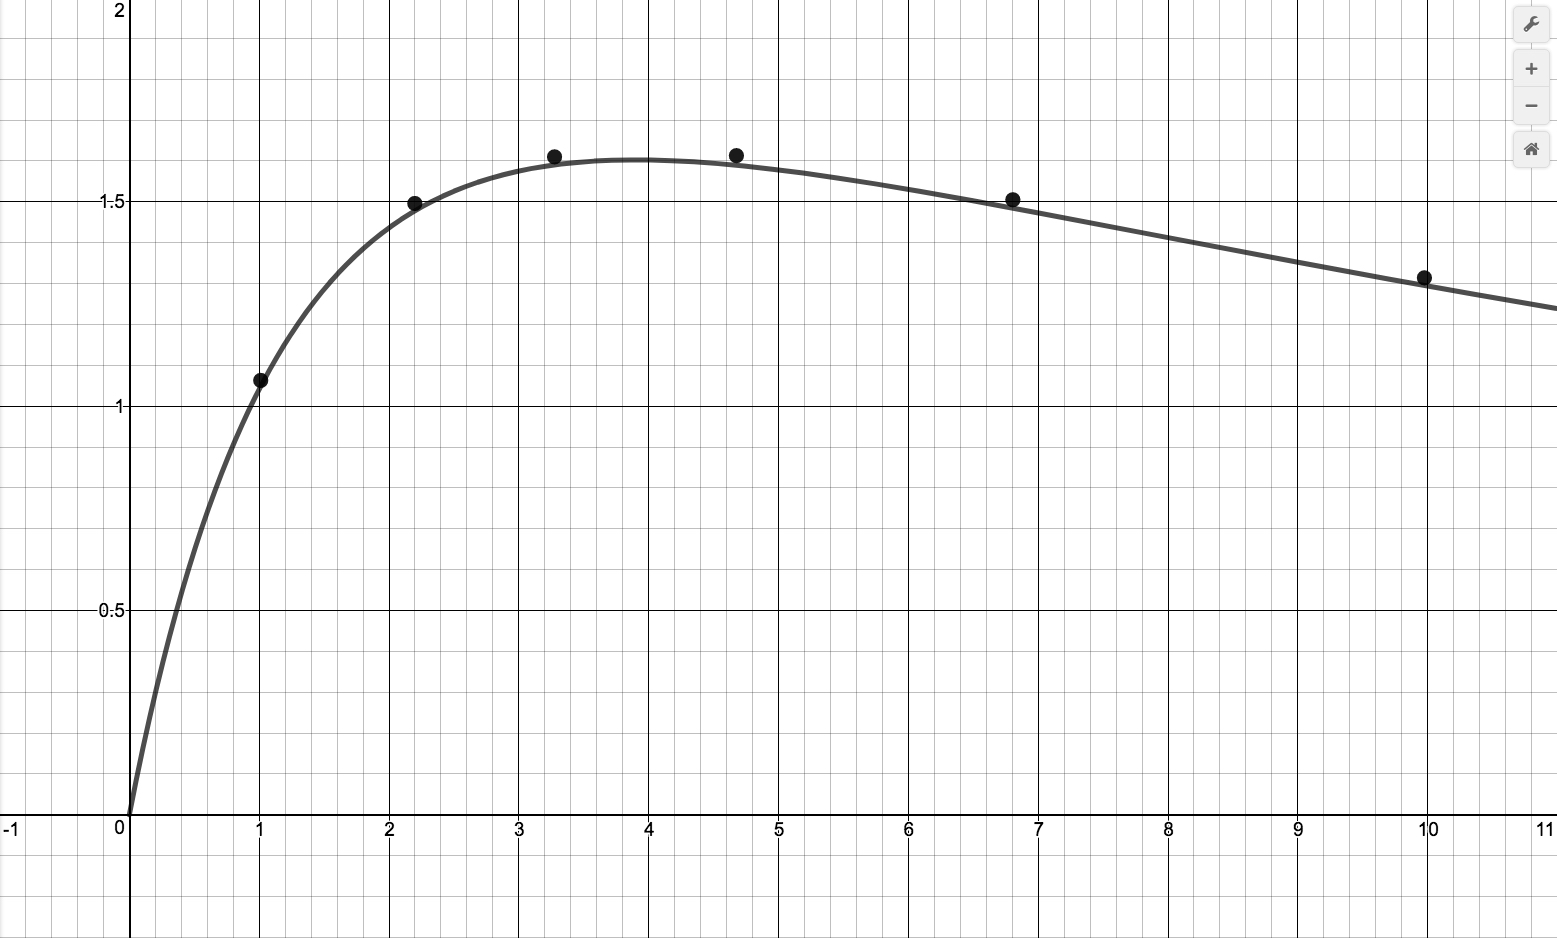
\includegraphics[height=2in]{./IntroRationalGraphics/MaxPowerRegression.jpg}

\item The maximum power is approximately $1.603 \; mW$ which corresponds to $3.9 \; k\Omega$.

\item As $x \rightarrow \infty, \; P(x) \rightarrow 0^{+}$ which means as the resistance increases without bound, the power diminishes to zero.

\end{enumerate}

\item  $a = -2$ and $c = -18$ so $f(x) = \dfrac{-2x^2+18}{x+3}$.

\item  \begin{multicols}{2}

 \begin{enumerate}

\item   $a=6$ and $n=2$ so $f(x) = \dfrac{6x^{2} -4}{2x^2+1}$

\item  $a=10$ and $n = 3$ so $f(x) = \dfrac{10x^{3} -4}{2x^2+1}$ .

\end{enumerate}
\end{multicols}


\item  If we define $f(x) = p(x) - p(a)$ then $f$ is a polynomial function with $f(a) = p(a) - p(a) = 0$.  The Factor Theorem guarantees $(x-a)$ is a factor of $f(x)$, that is, $f(x) = p(x) - p(a) = (x-a)q(x)$ for some polynomial $q(x)$. Hence, $r(x) = \frac{p(x)-p(a)}{x-a} = \frac{(x-a)q(x)}{x-a} = q(x)$ so the graph of $y = r(x)$ is the same as the graph of the polynomial $y = q(x)$ except for a hole when $x = a$.

\item  The slope of the curves near $x=1$ matches the exponent on $x$.  This exactly what we saw in  Exercise \ref{monomialarcexercise} in Section \ref{GraphsofPolynomials}.

\[ \begin{array}{|r||c|c|c|c|}  \hline

 f(x) &  [0.9, 1.1] & [0.99, 1.01] &[0.999, 1.001] & [0.9999, 1.0001]  \\ \hline
 x^{-1} & -1.0101 & -1.0001 & \approx -1 & \approx -1  \\  \hline
 x^{-2}& -2.0406& -2.0004 & \approx -2 & \approx -2   \\  \hline
 x^{-3} &-3.1021 & -3.0010 & \approx -3 & \approx -3   \\  \hline
 x^{-4} &-4.2057 & -4.0020 &\approx -4 & \approx -4   \\   \hline


\end{array} \]

\end{enumerate} 